\chapter{Rezultati}
V tem poglavju bom opisal rezultate, ki sem jih pridobil. Kot sem že omenil, bo večji del preizkušanja programa opravljen na slikah, kjer bodo nekateri piksli manjkali. Gre za problem, ki ga je moč lepo vizualizirati, saj pogosto pri surovih podatkih ni lahko definirati njihovo točnost, zaradi česar težko interpretiramo, kako koristen je sam algoritem.

Prav tako bom opisal točnost rezulatov različnih metod kot tudi čas izvajanja posameznih metod. Probleme bom zagnal tudi na različnih vrst podatkov, npr. podatkih ki so generirani normalno kot tudi enakomerno porazdeljeno.
Zaradi interpretacije, slike razdelimo v več skupin, za katere opišemo ugotovitve.

Vse slike si je mogoče v boljši kakovosti ogledati na povezavi \url{https://tinyurl.com/yb7cjdv7}. 

\section{Velika črno-bela slika}
Same teste algoritmov najprej poženemo na veliki, črno-beli sliki, velikosti $1000\times1000$ pikslov. Taka izbira je smiselna, iz vidika, da imamo dovolj podatkov, potrebnih za rekonstrukcijo. Ker je časovna zahtevnost algoritmov pri večjih slikah, kot bomo videli v nadaljevanju že precej velika, nam ta faza testiranja služi kot preverjanje delovanja samih algoritmov. Same podrobnosti razlik med rezultati si bomo zato podrobneje pogledali na manjših slikah v nadaljevanju. Algoritme preizkušamo trikrat, na podatkih z deleži znanih vrednosti $0.35, 0.45$ in $0.6$. \todo{Smiselna postavitev teskst-slik in velikosti}
\renewcommand{\mapa}{Poglavja/Slike/grayscale1000}

\begin{figure}[!ht]
    \centering
    \begin{subfigure}{0.49\linewidth}
        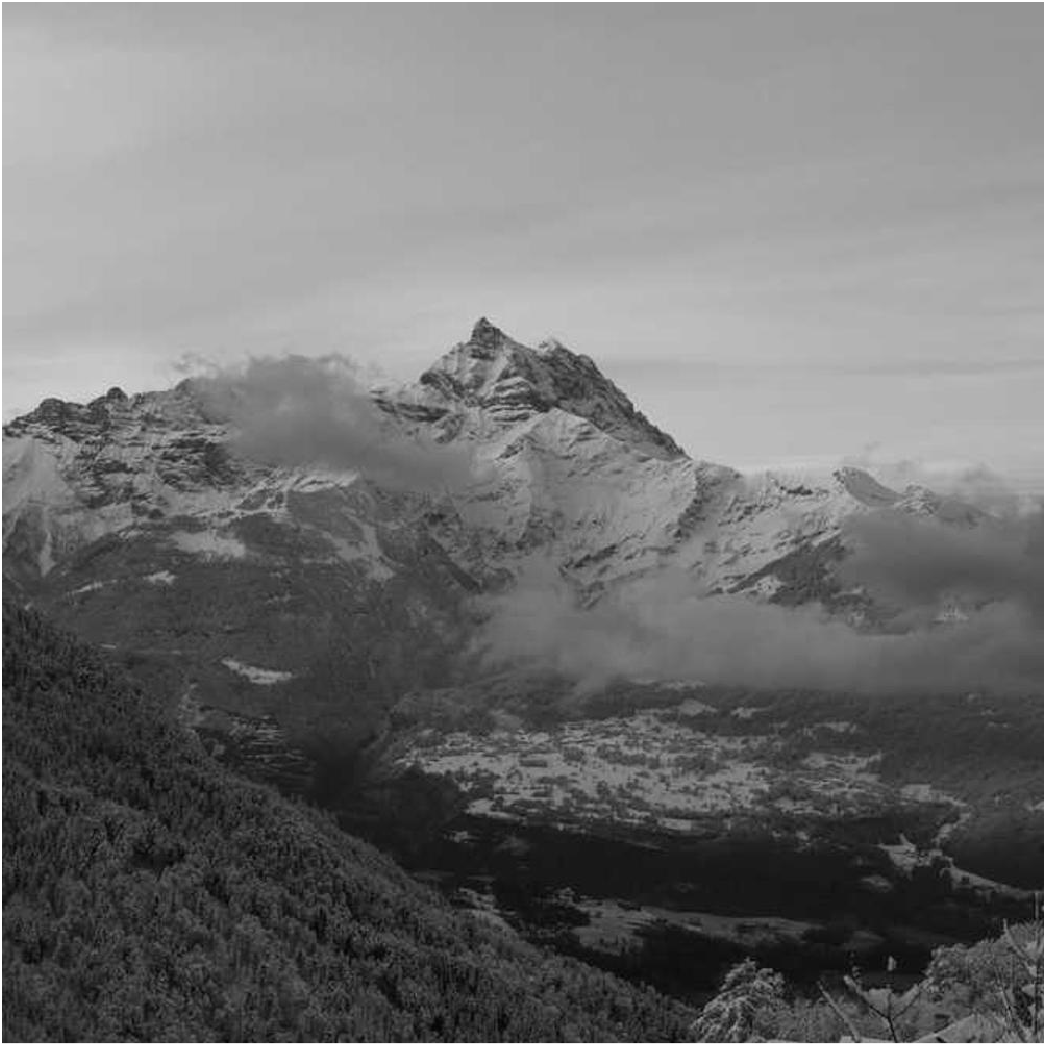
\includegraphics[width=\linewidth]{\mapa/slikaInput.png}
        \caption{Originalna slika.}
    \end{subfigure}
    \hfill
    \begin{subfigure}{0.49\linewidth}
        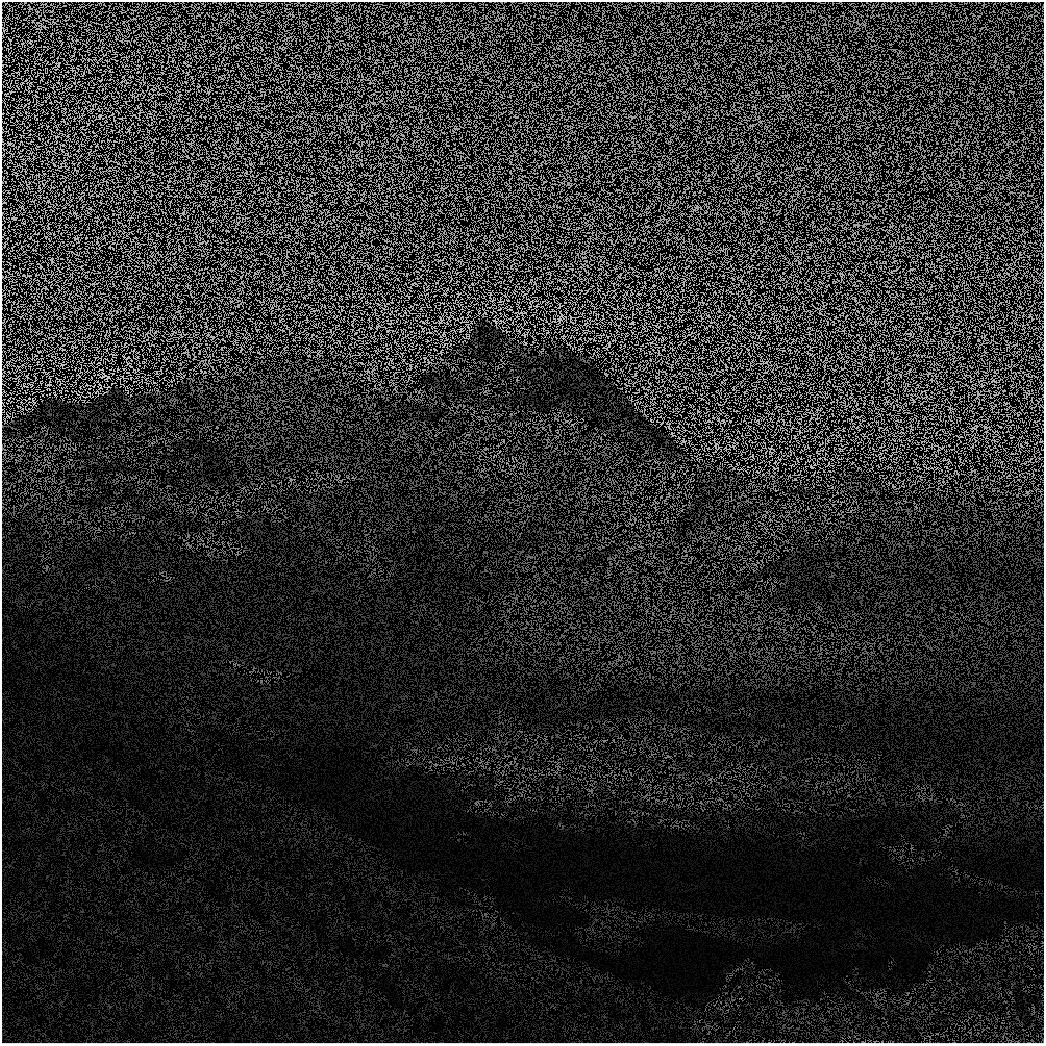
\includegraphics[width=\linewidth]{\mapa/slikaInput35.png}
        \caption{Slika z $35\%$ znanimi podatki.}
    \end{subfigure}
    \begin{subfigure}{0.49\linewidth}
        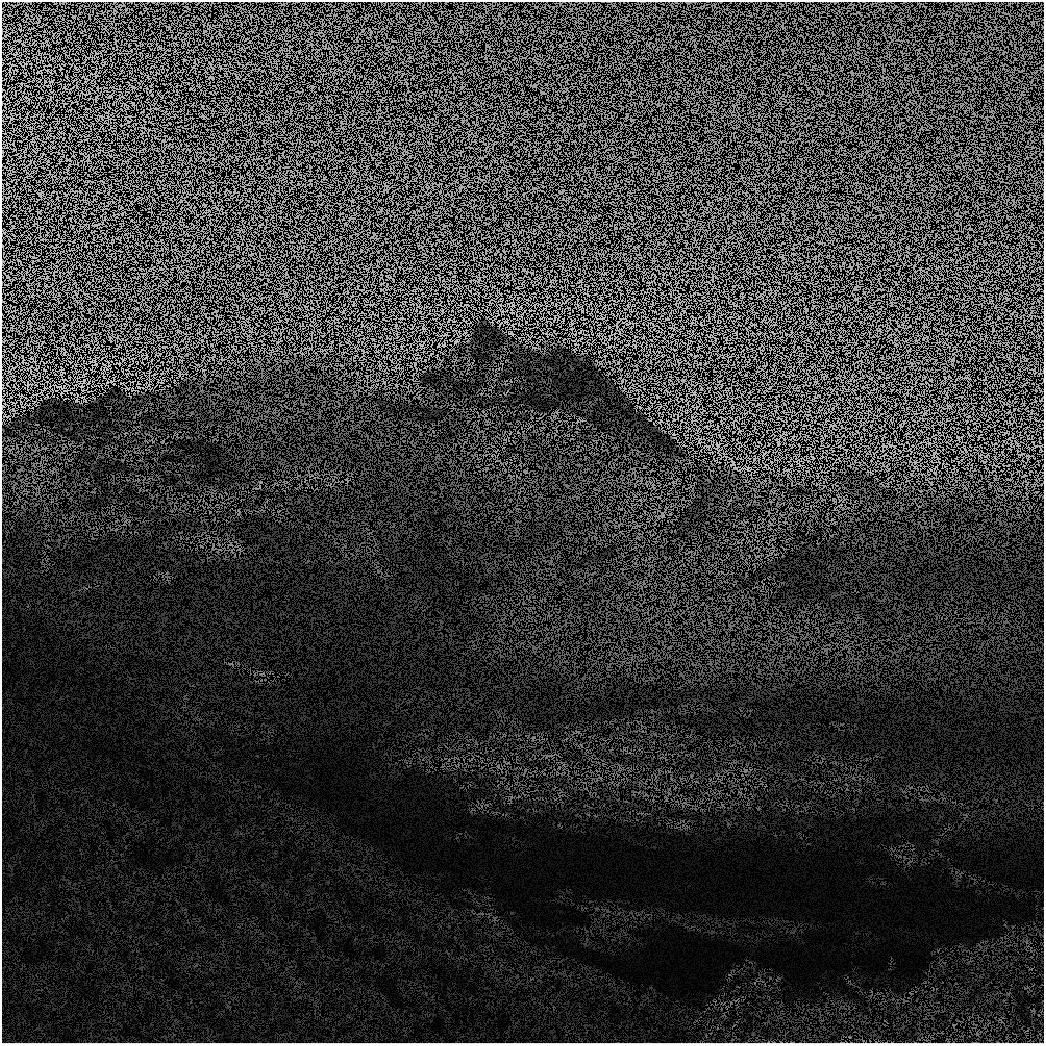
\includegraphics[width=\linewidth]{\mapa/slikaInput45.png}
        \caption{Slika z $45\%$ znanimi podatki.}
    \end{subfigure}
    \hfill
    \begin{subfigure}{0.49\linewidth}
        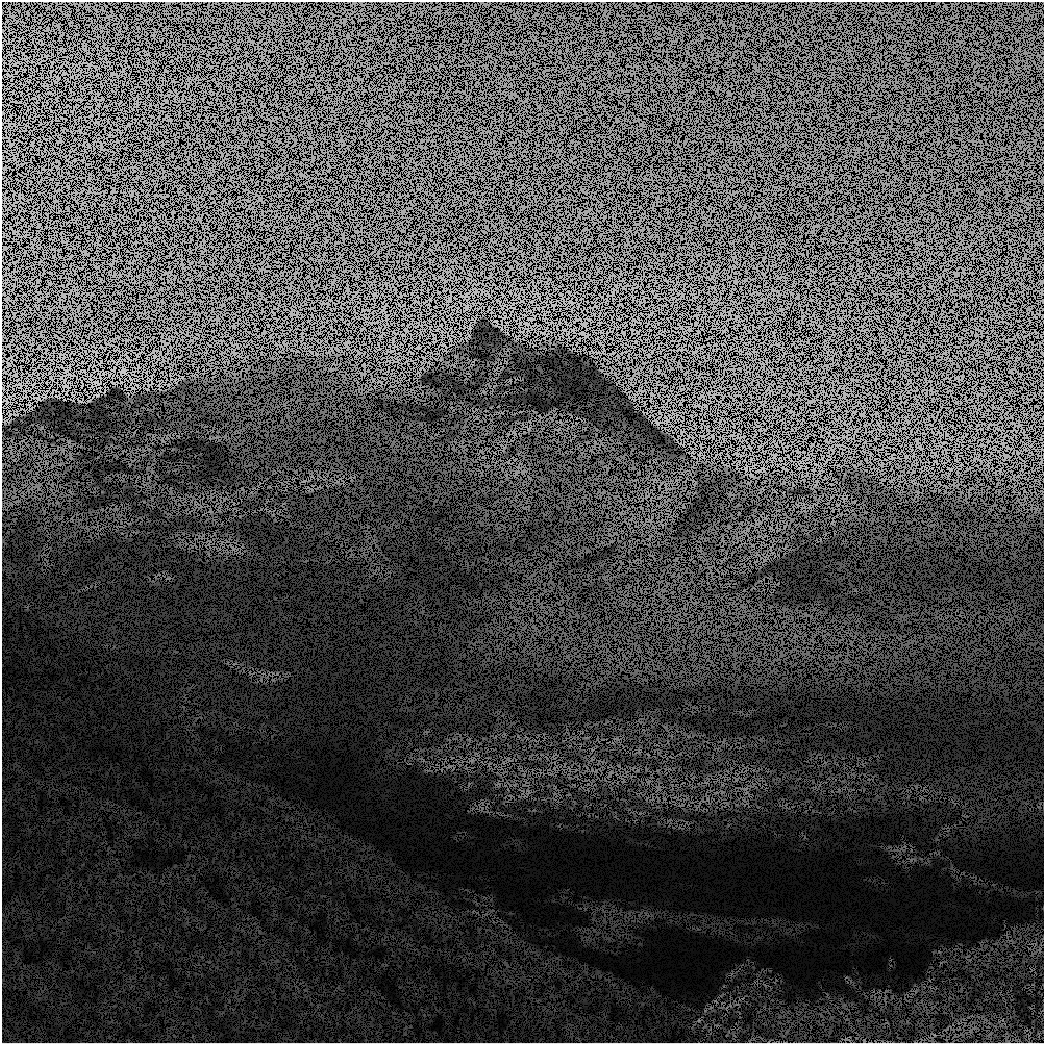
\includegraphics[width=\linewidth]{\mapa/slikaInput60.png}
        \caption{Slika z $60\%$ znanimi podatki.}
    \end{subfigure}
    \caption{Slika uporabljena za rekonstrukcijo. \cite{UnsplashGora}}
\end{figure}

\begin{figure}[!ht]
    \centering
    \begin{subfigure}{0.325\linewidth}
        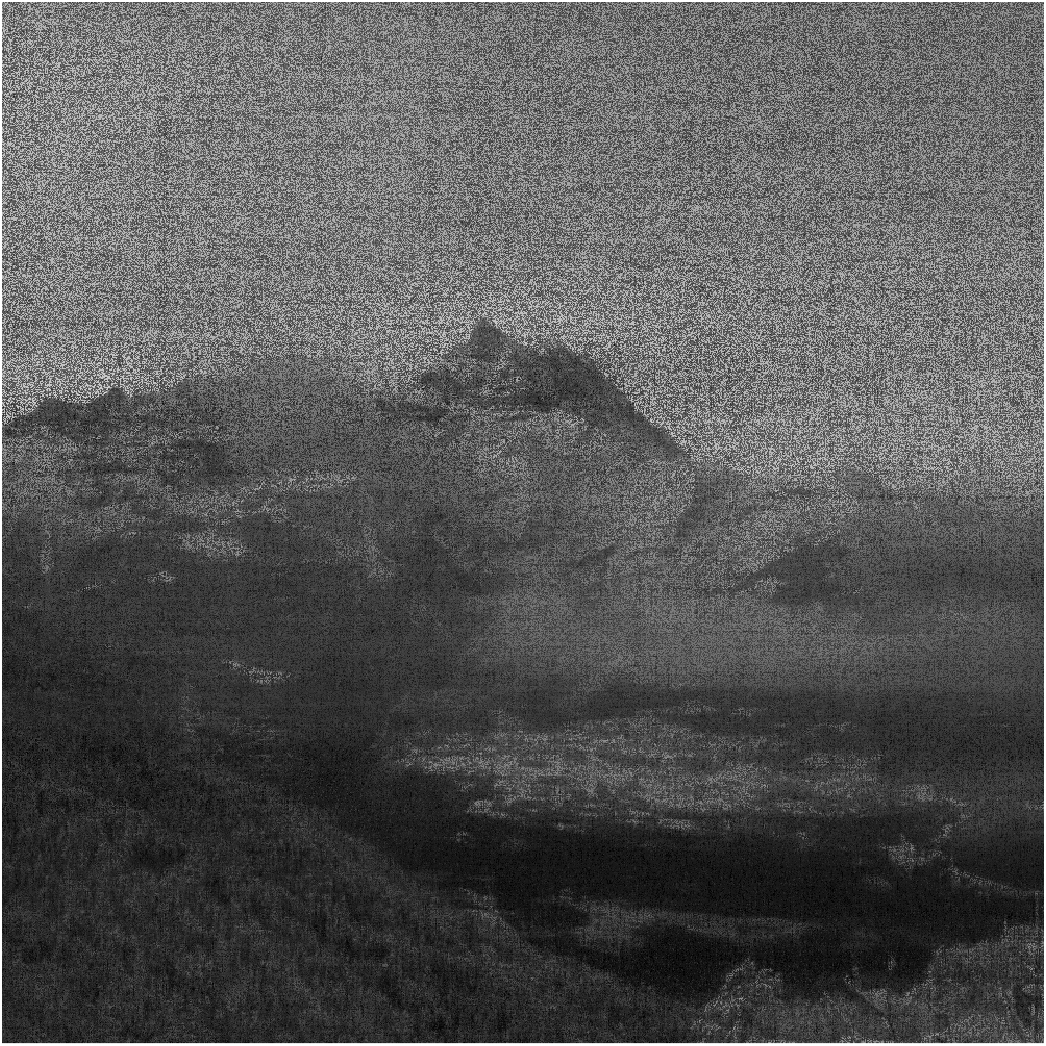
\includegraphics[width=\linewidth]{\mapa/slikaRez35SVT.png}
        \caption{SVT $35\%$}
    \end{subfigure}
    \hfill
    \begin{subfigure}{0.325\linewidth}
        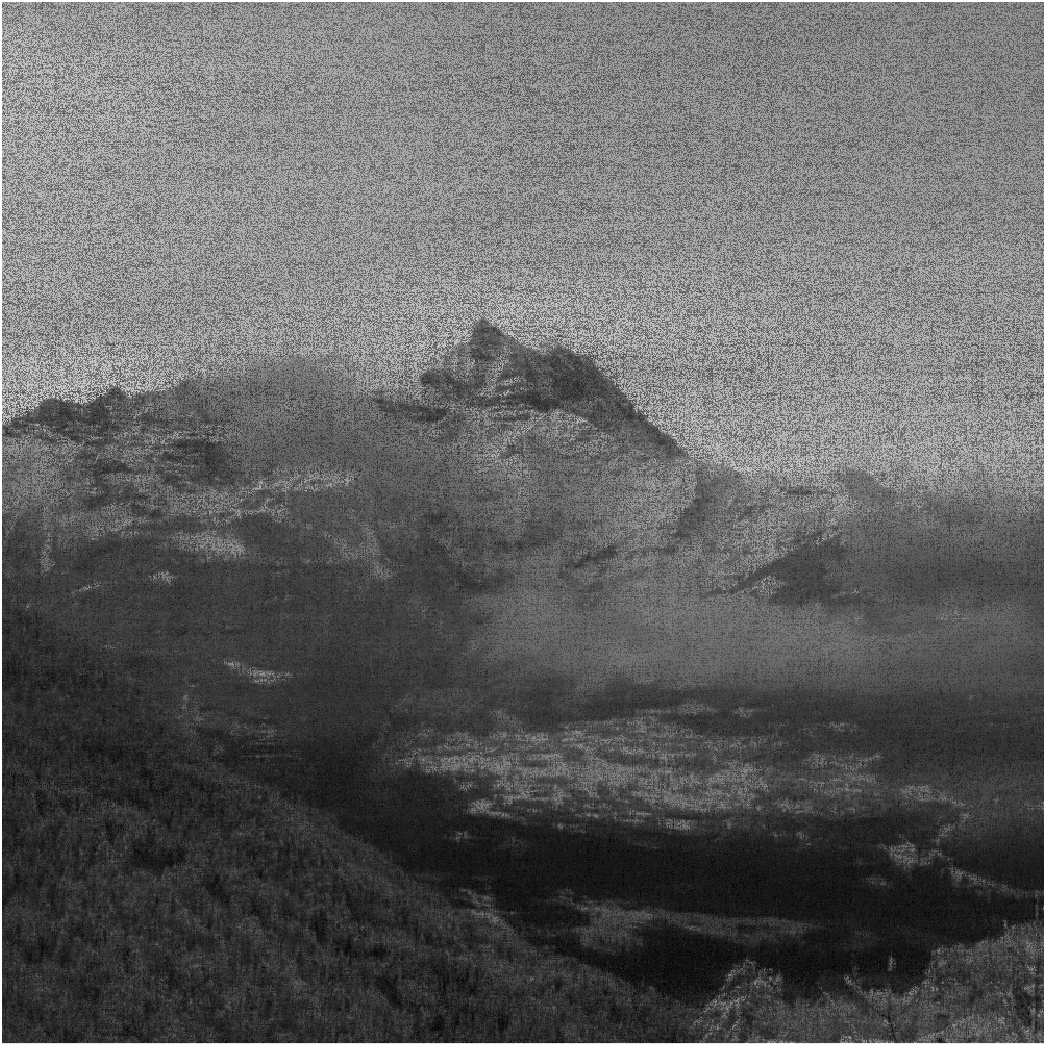
\includegraphics[width=\linewidth]{\mapa/slikaRez45SVT.png}
        \caption{SVT $45\%$}
    \end{subfigure}
    \hfill
    \begin{subfigure}{0.325\linewidth}
        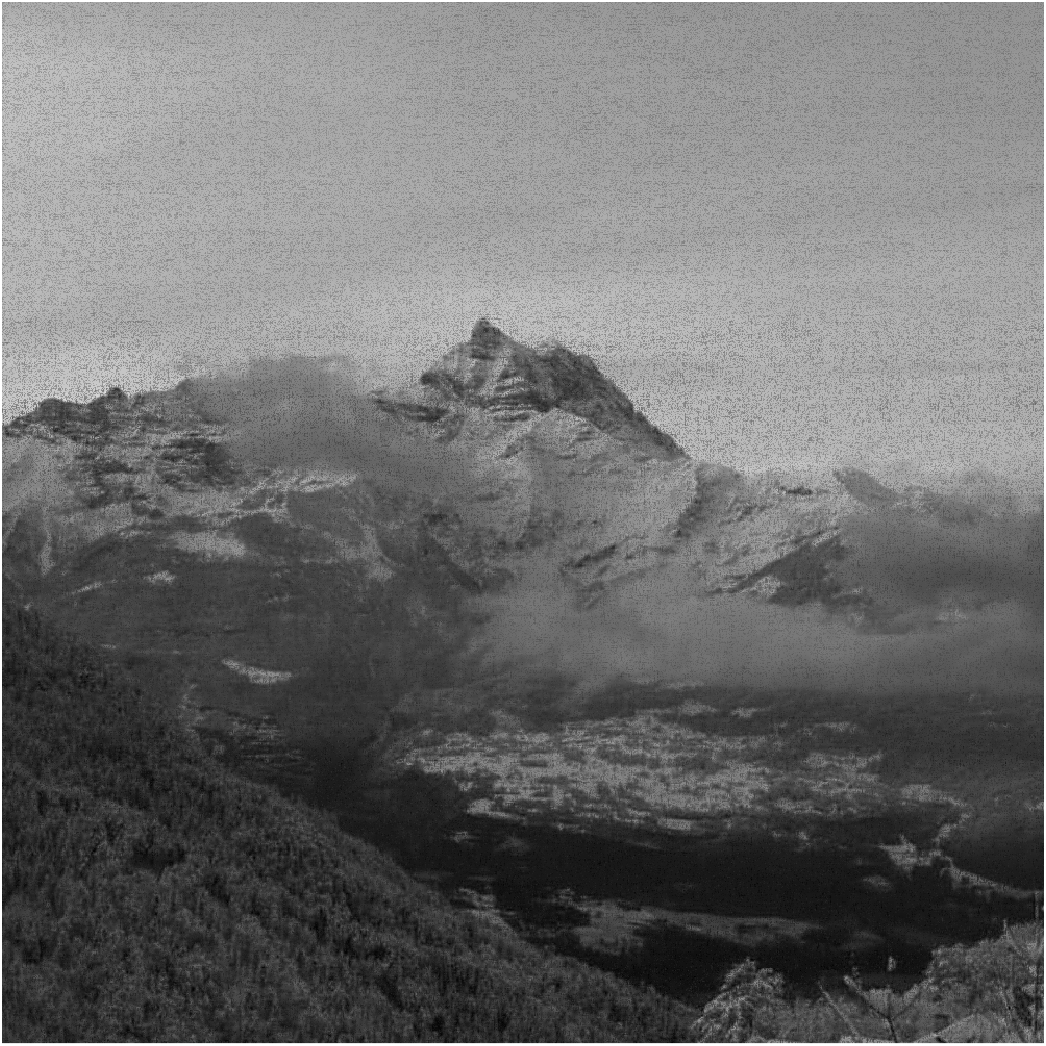
\includegraphics[width=\linewidth]{\mapa/slikaRez60SVT.png}
        \caption{SVT $60\%$}
    \end{subfigure}
    \begin{subfigure}{0.325\linewidth}
        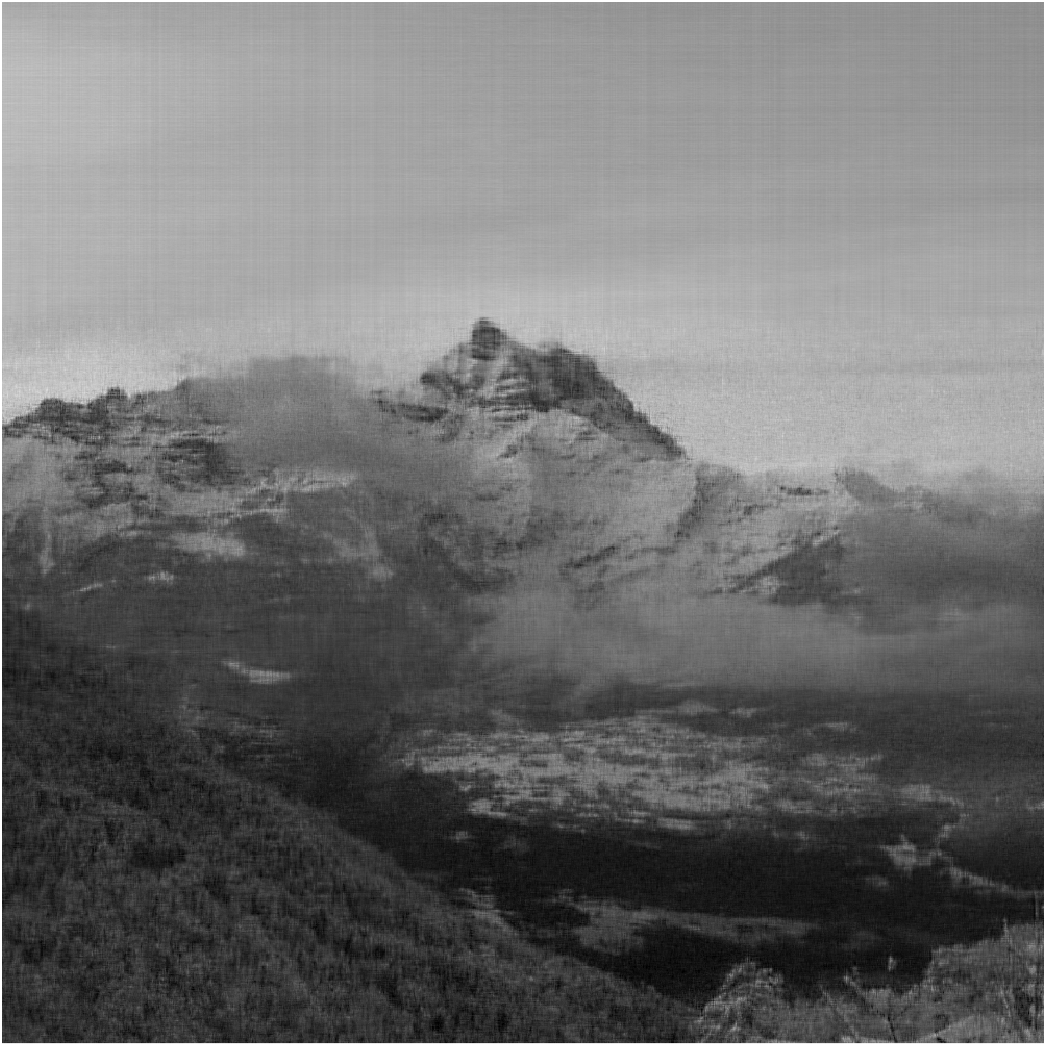
\includegraphics[width=\linewidth]{\mapa/slikaRez35TNNM.png}
        \caption{TNNM $35\%$}
    \end{subfigure}
    \hfill
    \begin{subfigure}{0.325\linewidth}
        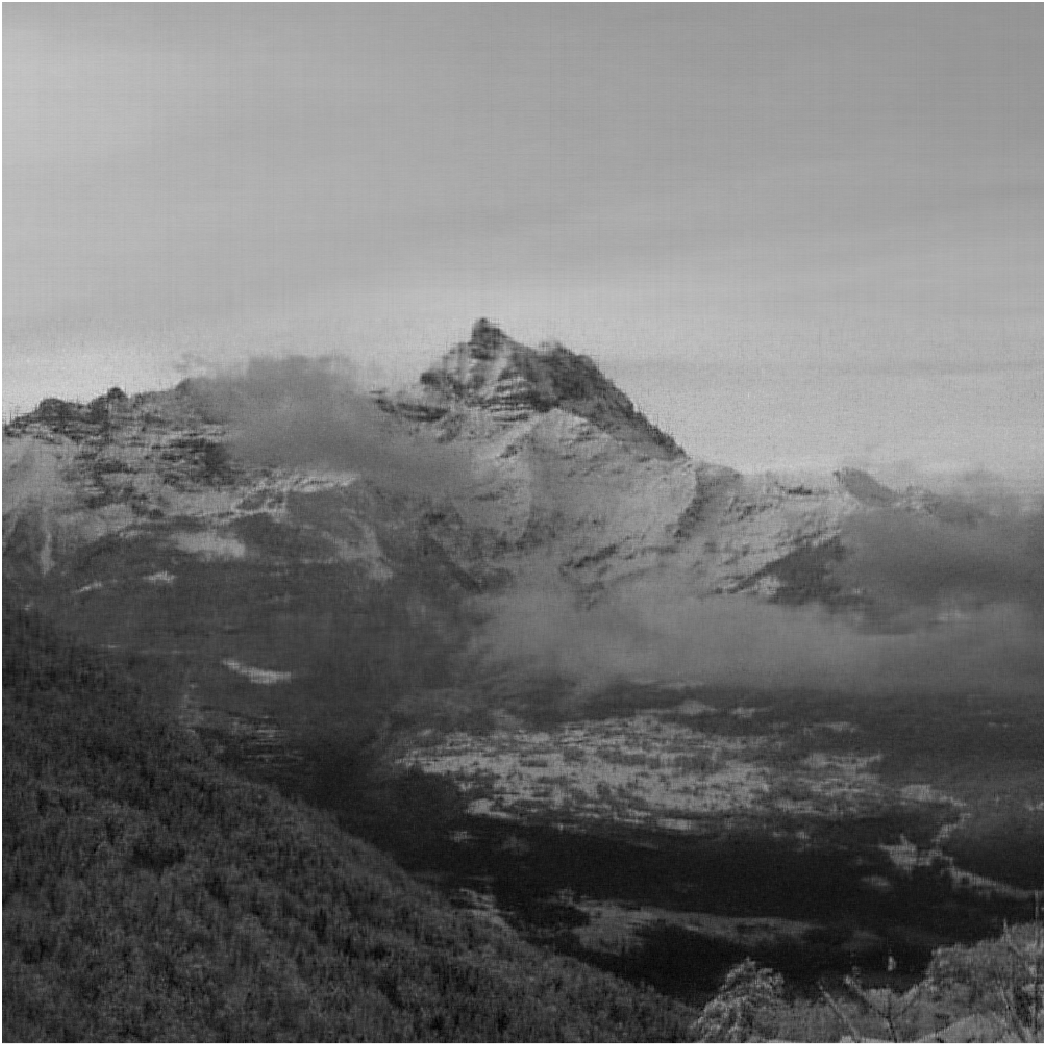
\includegraphics[width=\linewidth]{\mapa/slikaRez45TNNM.png}
        \caption{TNNM $45\%$}
    \end{subfigure}
    \hfill
    \begin{subfigure}{0.325\linewidth}
        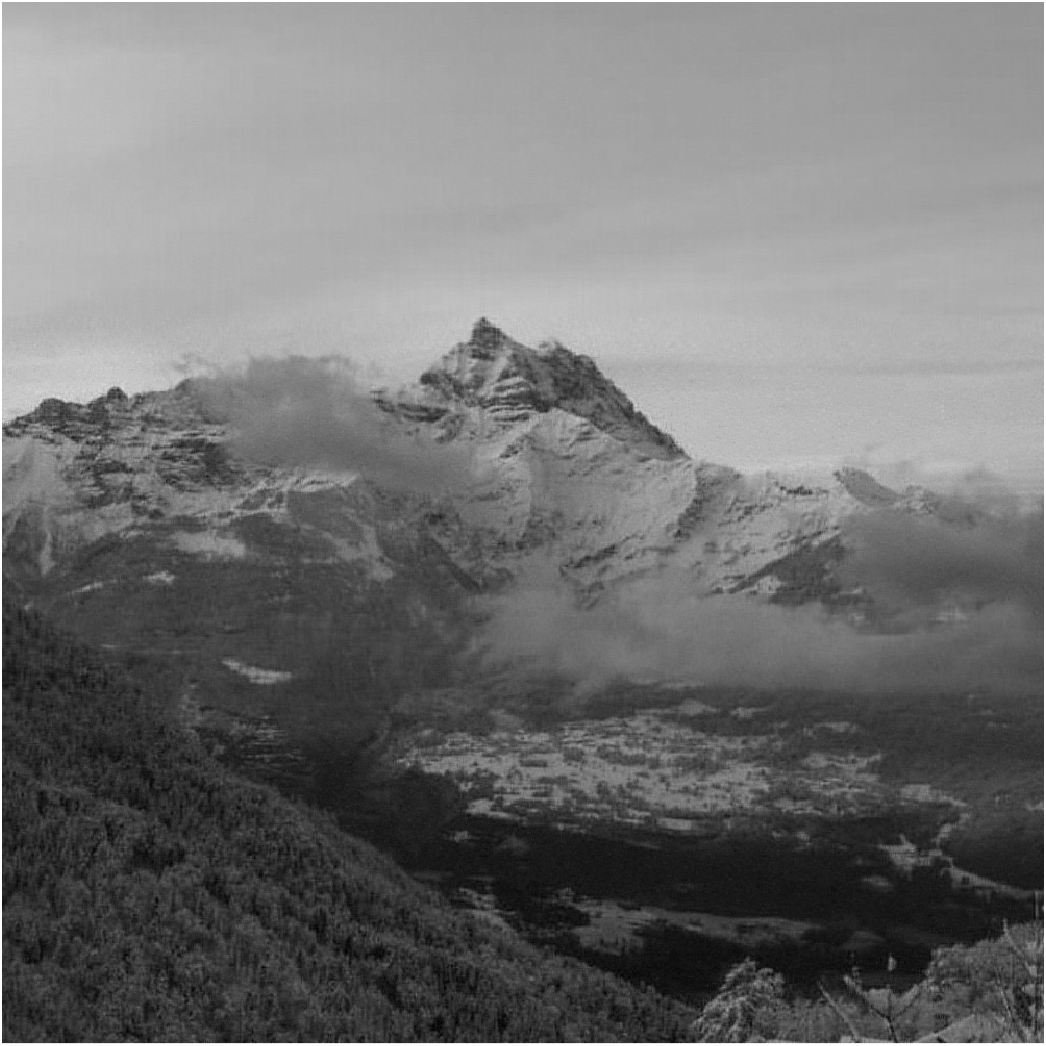
\includegraphics[width=\linewidth]{\mapa/slikaRez60TNNM.png}
        \caption{TNNM $60\%$}
    \end{subfigure}
    \begin{subfigure}{0.325\linewidth}
        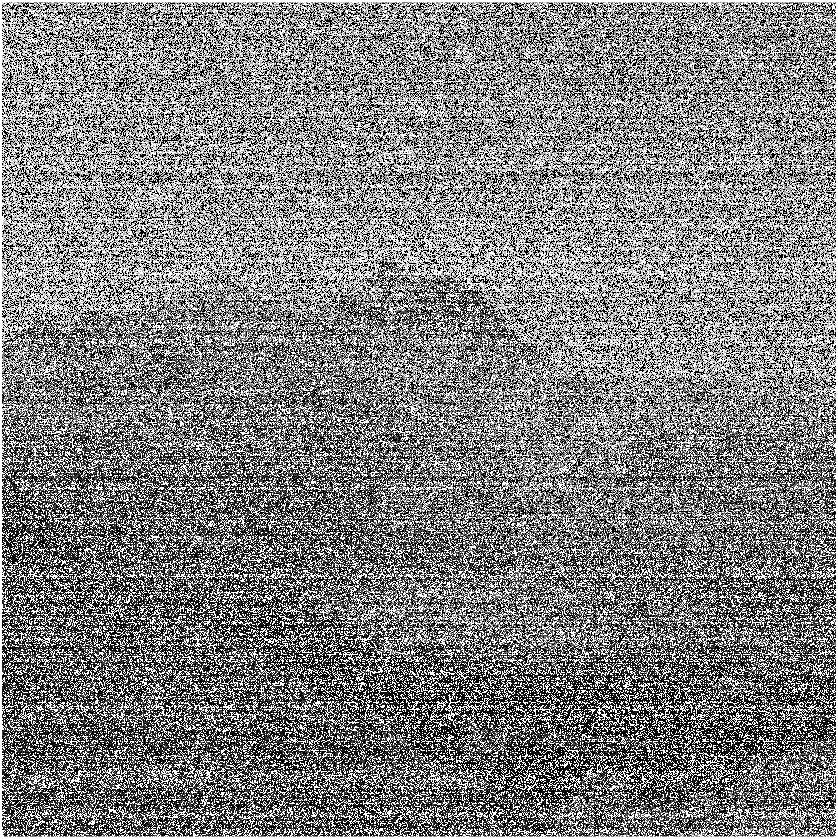
\includegraphics[width=\linewidth]{\mapa/slikaRez35ASD400.png}
        \caption{ASD $35\%$}
    \end{subfigure}
    \hfill
    \begin{subfigure}{0.325\linewidth}
        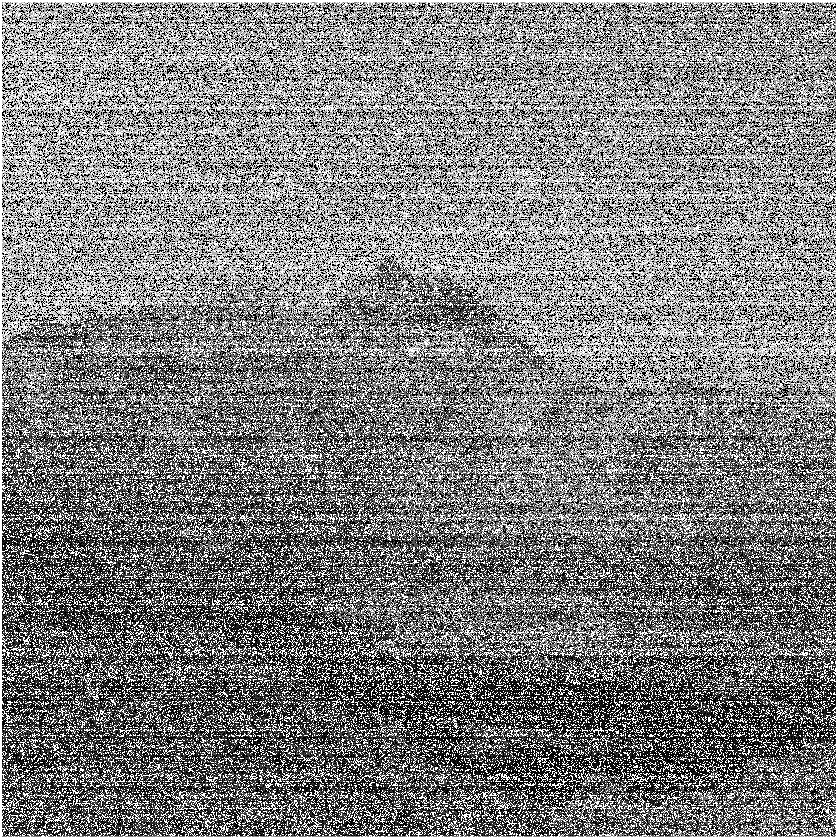
\includegraphics[width=\linewidth]{\mapa/slikaRez45ASD600.png}
        \caption{ASD $45\%$}
    \end{subfigure}
    \begin{subfigure}{0.325\linewidth}
        %ASD 60?%
        \hfill
    \end{subfigure}
    \begin{subfigure}{0.325\linewidth}
        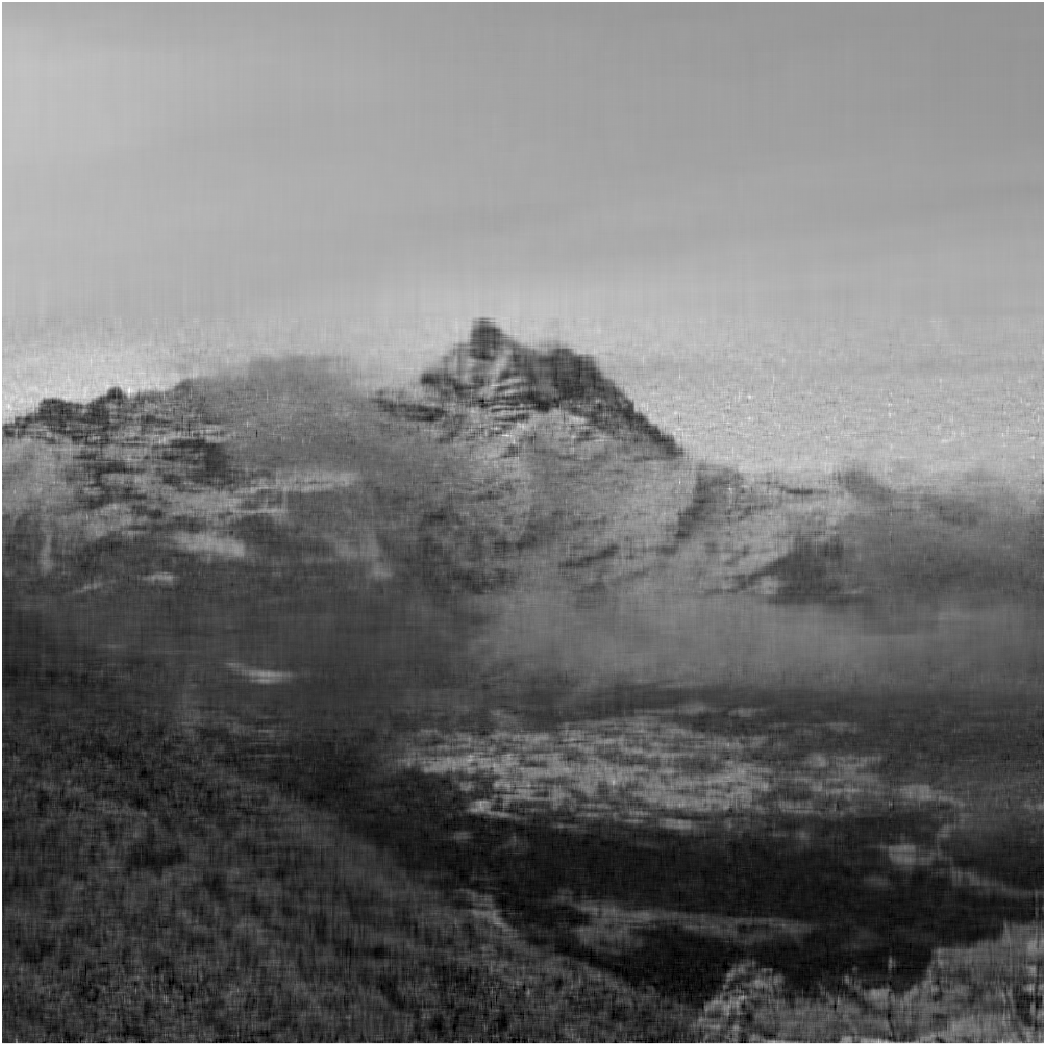
\includegraphics[width=\linewidth]{\mapa/slikaRez35LmaFIT50.png}
        \caption{LMaFit $35\%$}
    \end{subfigure}
    \hfill
    \begin{subfigure}{0.325\linewidth}
        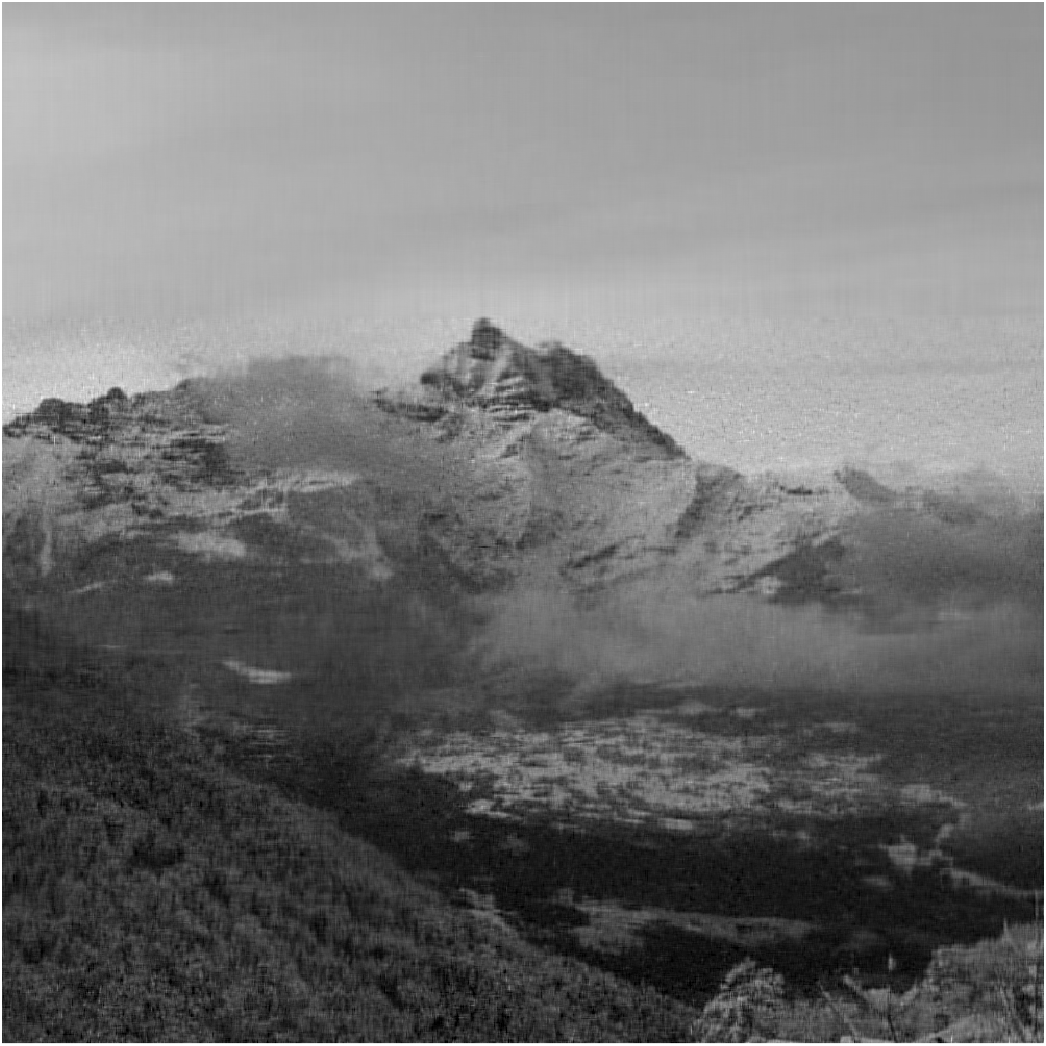
\includegraphics[width=\linewidth]{\mapa/slikaRez45LmaFIT73.png}
        \caption{LMaFit $45\%$}
    \end{subfigure}
    \begin{subfigure}{0.325\linewidth}
        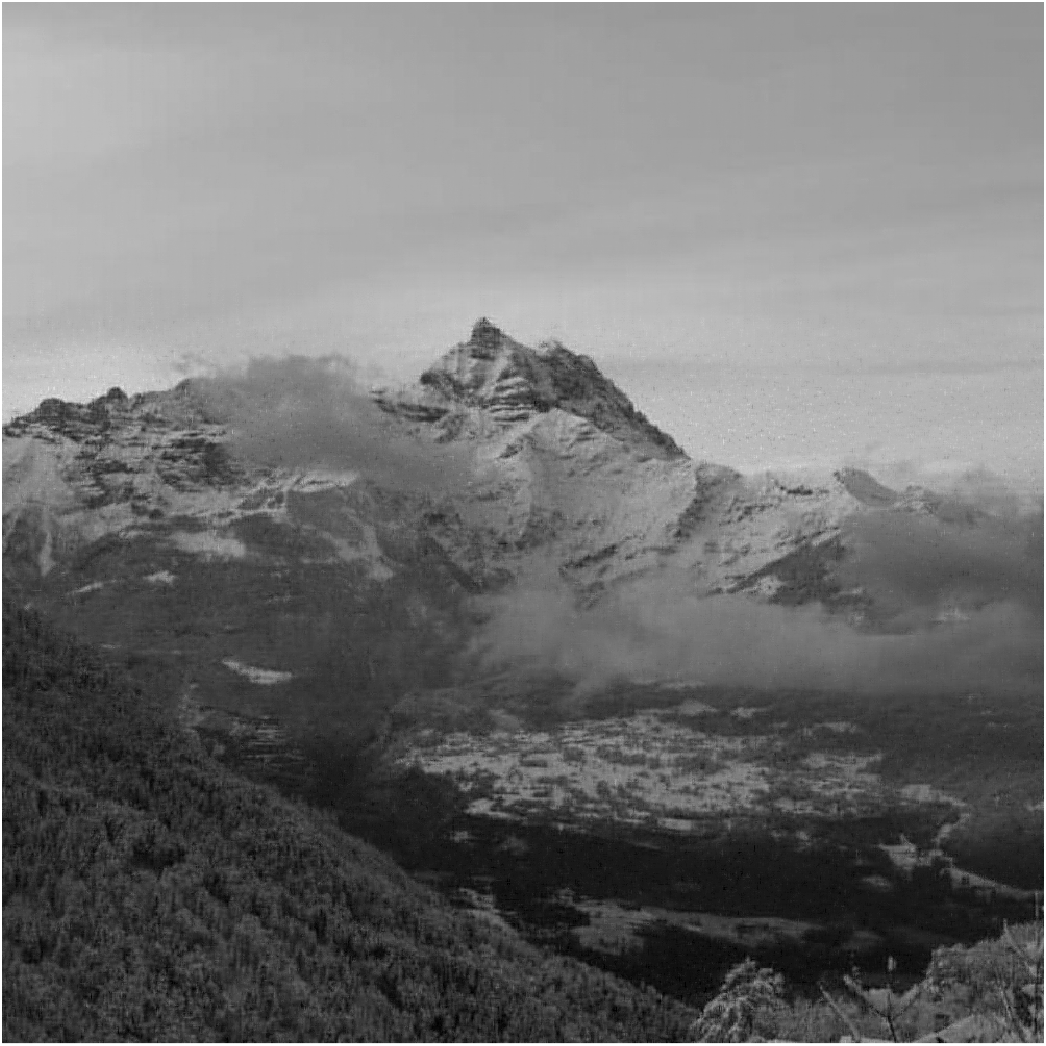
\includegraphics[width=\linewidth]{\mapa/slikaRez60LmaFIT77.png}
        \caption{LMaFit $60\%$}
    \end{subfigure}
\end{figure}
\FloatBarrier

Kot vidimo, je med rezultati velika razlika. Očitno je, da algoritmi TNNM, SVT in LMaFit delujejo najbolje, medtem ko ima algoritem ADDM vprašljive rezultate. Te si lahko interpretiramo kot posledico lastnosti, da lahko algoritem končata v lokalnem minimumu. Prav tako algoritem ADMM ni našel rešitve, ko je imel poznanih $0.60$ podatkov. Zato je ta algoritma smiselno uporabljati, kadar imamo dober začeten približek matrik $X$ in $Y$ ter manj poznanih vrednosti. Algoritem NNM smo med rezultati izpustili, saj je zaradi velikega števila matrik, potrebnih za definicijo omejitev, algoritem preveč prostorsko kompleksen. Ta algoritem bomo zato obravnavali posebej. Zaradi teh opazk se v naslednjih podpoglavjih v večini osredotočamo na algoritme SVT, TNNM in LMaFit.
\todo{je potrebno in graf in tabelo?}
\begin{table}[h]
    \centering
    \begin{tabular}{|c|c|c|c|c|}
    \hline
    & SVT & TNNM & LMAFIT & ASD \\ \hline
    0.35 & $4.69 \times 10^4$ & $7.70 \times 10^3$ & $8.03 \times 10^3$ & $3.9743 \times 10^7$ \\ \hline
    0.45 & $3.15 \times 10^4$ & $5.30 \times 10^3$ & $6.40 \times 10^3$ & $6.0910 \times 10^7$ \\ \hline
    0.6 & $1.25 \times 10^4$ & $3.58 \times 10^3$ & $5.35 \times 10^3$ & - \\ \hline
    \end{tabular}
\end{table}
\begin{figure}[!ht]
    \centering
    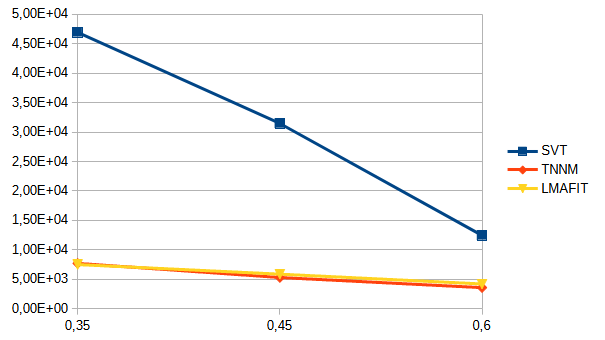
\includegraphics[width=\linewidth]{Poglavja/Slike/grayscale1000/grafNapake.png}
    \caption{Napake algoritmov glede na delež znanih vrednosti}
\end{figure}

\begin{table}[h]
    \centering
    \begin{tabular}{|c|c|c|c|c|}
    \hline
    & SVT & TNNM & LMAFIT & ASD \\ \hline
    0.35 & 338s & 824s & 235s & 1012s \\ \hline
    0.45 & 510s & 498s & 342s & 328s\\ \hline
    0.6 & 1674s & 350s & 48s & - \\ \hline
    \end{tabular}
\end{table}
\begin{figure}[!ht]
    \centering
    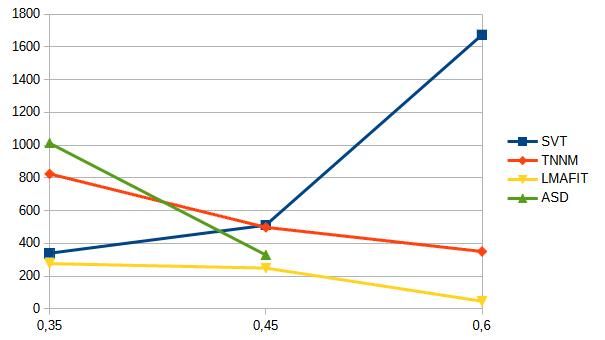
\includegraphics[width=\linewidth]{Poglavja/Slike/grayscale1000/grafCas.png}
    \caption{Časi izvajanja algoritmov glede na delež znanih vrednosti}
\end{figure}

\section{Vpliv kompleksnosti slik na napolnjevanje}
Eno izmed glavnih vprašanj, ki se nam lahko porodi pri implementaciji algoritmov za napolnitev matrik je, kako sama kompleksnost slik vpliva na točnost rezultatov. Ker slike naključnih vrednosti ni mogoče rekonstruirati, lahko sklepamo, da bodo slike s preprostimi motivi napolnjene bolje. Za namene testiranja je torej smiselno izbrati tako preprosto kot tudi vizualno nasičeno sliko. V naših testiranjih uporabljamo sliki knjige in mesta. Sliki sta velikosti $300 \times 300$ pikslov
\renewcommand{\mapa}{Poglavja/Slike/kompleksnost}

\begin{figure}[!ht]
    \begin{subfigure}{0.5\linewidth}
        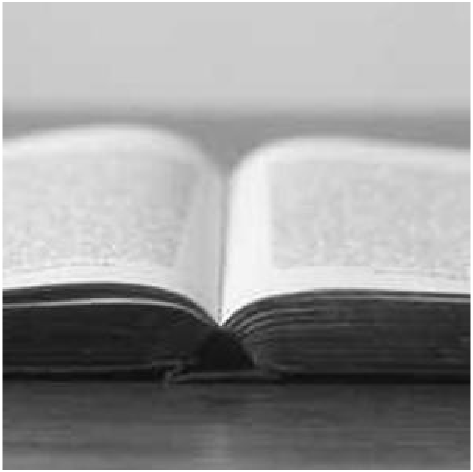
\includegraphics[width=\linewidth]{\mapa/preprosta grayscale 300/knjiga.png}
        \caption{Slika s preprostim motivom.}
    \end{subfigure}
    \hfill
    \begin{subfigure}{0.5\linewidth}
        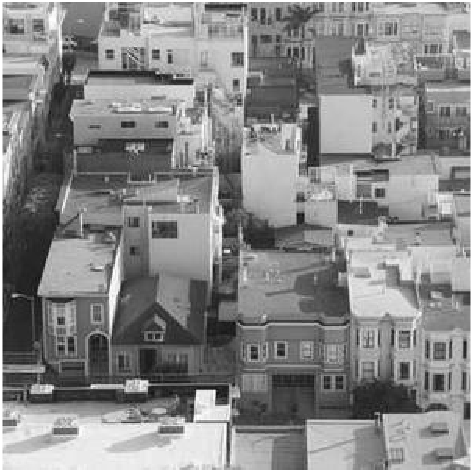
\includegraphics[width=\linewidth]{\mapa/kompleksna grayscale 300/mesto.png}
        \caption{Slika s kompleksnim motivom.}
    \end{subfigure}
    \caption{Vira slik: \cite{UnsplashKnjiga,UnsplashMesto}.}
\end{figure}

\begin{figure}[!ht]
    \begin{subfigure}{0.325\linewidth}
        \includegraphics[width=\linewidth]{\mapa/preprosta grayscale 300/rez35SVT.png}
    \end{subfigure}
    \hfill
    \begin{subfigure}{0.325\linewidth}
        \includegraphics[width=\linewidth]{\mapa/preprosta grayscale 300/rez45SVT.png}
    \end{subfigure}
    \hfill
    \begin{subfigure}{0.325\linewidth}
        \includegraphics[width=\linewidth]{\mapa/preprosta grayscale 300/rez60SVT.png}
    \end{subfigure}
    \caption{Rekonstrukcija preprostega motiva z algoritmom SVT. Odstotki znanih vrednosti slik so bili 35\% (leva), 45\% (sredinska) in 60\% (desna).
    }
\end{figure}
    
\begin{figure}[!ht]
    \begin{subfigure}{0.325\linewidth}
        \includegraphics[width=\linewidth]{\mapa/kompleksna grayscale 300/rez35SVT.png}
    \end{subfigure}
    \hfill
    \begin{subfigure}{0.325\linewidth}
        \includegraphics[width=\linewidth]{\mapa/kompleksna grayscale 300/rez45SVT.png}
    \end{subfigure}
    \hfill
    \begin{subfigure}{0.325\linewidth}
        \includegraphics[width=\linewidth]{\mapa/kompleksna grayscale 300/rez60SVT.png}
    \end{subfigure}
    \caption{Rekonstrukcija kompleksnega motiva z algoritmom SVT. Odstotki znanih vrednosti slik so bili 35\% (leva), 45\% (sredinska) in 60\% (desna).}
\end{figure}

\begin{figure}[!ht]
    \begin{subfigure}{0.325\linewidth}
        \includegraphics[width=\linewidth]{\mapa/preprosta grayscale 300/rez35TNNM.png}
    \end{subfigure}
    \hfill
    \begin{subfigure}{0.325\linewidth}
        \includegraphics[width=\linewidth]{\mapa/preprosta grayscale 300/rez45TNNM.png}
    \end{subfigure}
    \hfill
    \begin{subfigure}{0.325\linewidth}
        \includegraphics[width=\linewidth]{\mapa/preprosta grayscale 300/rez60TNNM.png}
    \end{subfigure}
    \caption{Rekonstrukcija preprostega motiva z algoritmom TNNM. Odstotki znanih vrednosti slik so bili 35\% (leva), 45\% (sredinska) in 60\% (desna).}
\end{figure}

\begin{figure}[!ht]
    \begin{subfigure}{0.325\linewidth}
        \includegraphics[width=\linewidth]{\mapa/kompleksna grayscale 300/rez35TNNM.png}
    \end{subfigure}
    \hfill
    \begin{subfigure}{0.325\linewidth}
        \includegraphics[width=\linewidth]{\mapa/kompleksna grayscale 300/rez45TNNM.png}
    \end{subfigure}
    \hfill
    \begin{subfigure}{0.325\linewidth}
        \includegraphics[width=\linewidth]{\mapa/kompleksna grayscale 300/rez60TNNM.png}
    \end{subfigure}
    \caption{Rekonstrukcija kompleksnega motiva z algoritmom TNNM. Odstotki znanih vrednosti slik so bili 35\% (leva), 45\% (sredinska) in 60\% (desna).}
\end{figure}

\begin{figure}[!ht]
    \begin{subfigure}{0.325\linewidth}
        \includegraphics[width=\linewidth]{\mapa/preprosta grayscale 300/rez35LMaFit.png}
    \end{subfigure}
    \hfill
    \begin{subfigure}{0.325\linewidth}
        \includegraphics[width=\linewidth]{\mapa/preprosta grayscale 300/rez45LMaFit.png}
    \end{subfigure}
    \hfill
    \begin{subfigure}{0.325\linewidth}
        \includegraphics[width=\linewidth]{\mapa/preprosta grayscale 300/rez60LMaFit.png}
    \end{subfigure}
    \caption{Rekonstrukcija preprostega motiva z algoritmom LMaFit. Odstotki znanih vrednosti slik so bili 35\% (leva), 45\% (sredinska) in 60\% (desna).}
\end{figure}

\begin{figure}[!ht]
    \begin{subfigure}{0.325\linewidth}
        \includegraphics[width=\linewidth]{\mapa/kompleksna grayscale 300/rez35LMaFit.png}
    \end{subfigure}
    \hfill
    \begin{subfigure}{0.325\linewidth}
        \includegraphics[width=\linewidth]{\mapa/kompleksna grayscale 300/rez45LMaFit.png}
    \end{subfigure}
    \hfill
    \begin{subfigure}{0.325\linewidth}
        \includegraphics[width=\linewidth]{\mapa/kompleksna grayscale 300/rez60LMaFit.png}
    \end{subfigure}
    \caption{Rekonstrukcija preprostega motiva z algoritmom LMaFit. Odstotki znanih vrednosti slik so bili 35\% (leva), 45\% (sredinska) in 60\% (desna).}
\end{figure}
\todo{Lmafit vcasih potrebno zagnati veckat}
\begin{figure}[!ht]
    \centering
    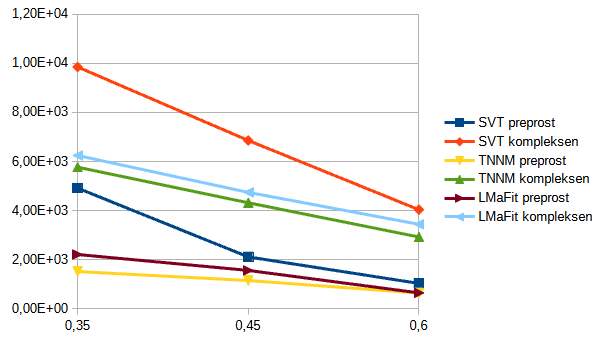
\includegraphics[width=\linewidth]{Poglavja/Slike/kompleksnost/kompleksna grayscale 300/kompleksnost.png}
    \caption{Graf napak algoritmov}
\end{figure}

Kot smo pričakovali, so rezultati rekonstrukcije slike s preprostim motivom boljše. Prav tako lahko opazimo, da ima delež znanih vrednosti močnejši vpliv pri sliki s kompleksnim motivom. Napake z dodajanjem informacij torej hitreje padajo pri matrikah večjega ranga. Spomnimo se, da algoritma LMaFit in TNNM za svoje delovanje potrebujeta informacijo o rangu. Pri testiranju je bilo zato potrebno kompleksni sliki podati večjo vrednost ranga, da sta lahko algoritma prišla do dobrih rezultatov.

Sama točnost algoritmov pa ostaja zelo podobna rekonstrukciji velike slike, torej z najboljšimi rezultati pridobljenimi z algoritmom TNNM, nato LMaFit in z najslabšimi rezultati algoritem SVT.

\begin{figure}[!ht]
    \centering
    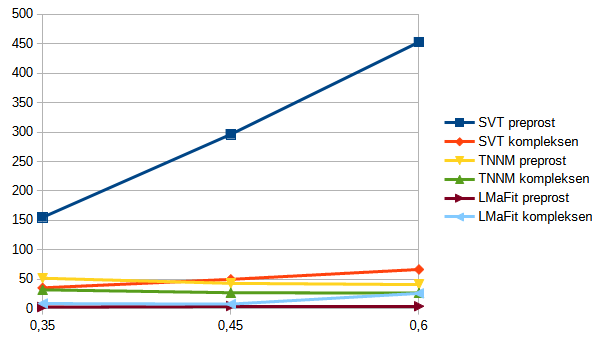
\includegraphics[width=\linewidth]{Poglavja/Slike/kompleksnost/kompleksna grayscale 300/cas.png}
    \caption{Graf časov izvajanja algoritmov}
\end{figure}
Sami časi izvajanja pa tu niso tako intuitivni. Prva glavna opazka je, da algoritem SVT potrebuje veliko več časa pri preprostem motivu kot pri kompleksem. \todo{razmisli to interpretacijo} To si lahko razlagamo kot posledico praga. Za dobre rezultate smo pri tako majhni matriki prag nastavili visoko. V našem primeru je imel ta vrednost $3600$. V primeru preprostega motiva, lahko pričakujemo, da bomo imeli malo zelo velikih singularnih vrednosti. Zaradi tega se algoritem težko premika in išče rešitev. Iz tega sledi opazka, da je algoritem SVT bolj smiselno uporabljati za kompleksne motive.

Naslednja pomembna opazka pa je, da delež znanih vrednosti različno vpliva na sam čas izvajanja. Tudi ta faktor je torej lahko pomemben pri izbiri algoritma za reševanje problema. Algoritem SVT potrebuje za rekonstrukcijo več časa, kadar ima poznanih več vrednosti, medtem ko se algoritmu TNNM z deležem znanih vrednosti čas izvajanja manjša. Algoritmu LMaFit težko določimo pravilo, saj najpočasnejše izvede rekonstrukcijo pri $0.45$ znanih podatkov. Iz tega sklepamo, da je pri nekem deležu med $0.35$ in $0.6$ rekonstrukcija najpočasnejša. Tu pa je vredno tudi omeniti, da zaradi naključnega generiranja začetne matrike algoritem lahko različno dolgo rekonstruira isti primer. \todo{Preveri znova} Ker pa smo teste pognali večkrat ter v povprečju vedno najdlje čakali pri vrednosti $0.45$ lahko sklepamo, da je v takih primerih rekonstrukcija res bolj zahtevna.

\section{Rekonstrukcija barvnih slik}
Naslednje vprašanje, ki se nam lahko porodi pri testiranju algoritmov je, kako vplivajo barvne slike na samo rekonstrukcijo. Barvne slike so podatkovno podane kot kombinacija barvnih kanalov rdeče, zelene in modre barve. Glavno vprašanje, na katerega bomo poskušali odgovoriti v tem poglavju je, ali je bolje napolnjevati vsak barvni kanal posebej, ali sliko kot celotno. V prvem primeru torej algoritem zaženemo trikrat, medtem ko v drugem sestavimo veliko matriko sestavljeno kot 
\[
    A = \begin{bmatrix}
        R\\G\\B
    \end{bmatrix} 
\] 
kjer $R$ predstavlja matriko z vrednostmi rdečega kanala, G vrednosti zelenega kanala ter B vrednosti modrega kanala.
Vsi testi v tej fazi so bili izvedeni na podatkih, kjer imamo poznanih $0.35$ informacij.
\todo{kako omeniti da je frobenius}
\begin{table}[h]
    \centering
    \begin{tabular}{|c|c|c|c|}
    \hline
    & SVT & TNNM & LMAFIT \\
    \hline
    Enojna rekonstrukcija & $1,50 \times 10^4$ & $9,60\times 10^3$ & $1,15\times 10^4$ \\
    Trojna rekonstrukcija & $1,66\times 10^4$ & $9,79\times 10^3$ & $1,14\times 10^4$ \\
    \hline
    \end{tabular}
\end{table}

\begin{table}[h]
    \centering
    \begin{tabular}{|c|c|c|c|}
    \hline
    & SVT & TNNM & LMAFIT \\
    \hline
    Enojna rekonstrukcija & 352s & 124s & 66s \\
    Trojna rekonstrukcija & 112s & 100s & 42s \\
    \hline
    \end{tabular}
\end{table}
Lahko je videti, da medtem ko obe metodi vrnete približno enako dobre rezultate, je rekonstrukcija pri vseh algoritmih hitrejša, če ločene barvne kanale rekonstruiramo posebej. Iz tu je lahko videti, da je smiselno med sabo neodvisne podatke ločiti, ter jih reševati samostojno. Rezultat je smiselen, saj nam iskanje podobnosti med nepodobnimi podatki poveča količino dela. 

\section{Vpliv podatka o rangu na rezultate}
Kot smo omenili že nekajkrat, algoritma TNNM in LMaFit za svoje izvajanje potrebujeta informacijo o rangu (v nadaljevanju parameter). V tem podpoglavju bomo poskušali odgovoriti na vprašanje, kako pri obeh algoritmih ta informacija vpliva na same rezultate in izvajanje. Za namene testiranja smo algoritem na isti sliki pognali večkrat, ter postopoma večali rang. Ponovno smo teste izvajali na sliki mesta, z znanim deležem podatkov nastavljenim na $0,35$.

\subsection{LMaFit}
V tej fazi smo algoritem testirali šestkrat, z rangom rezultata določenega na
$1, 5, 10, 22, 25$ in $60$. Vrednost $22$ je bila izbrana, ker je ob večkratnem zagonu programa na različnih parametrih, ta dala najboljši rezultat. Posledično sta bili vrednosti $25$ in $60$ izbrani z namenom opazovanja, kakšne rezultate pridobimo s precenitvijo ranga rekonstruirane matrike. 
\renewcommand{\mapa}{Poglavja/Slike/informacija ranga}

\begin{figure}[!ht]
    \begin{subfigure}{0.325\linewidth}
        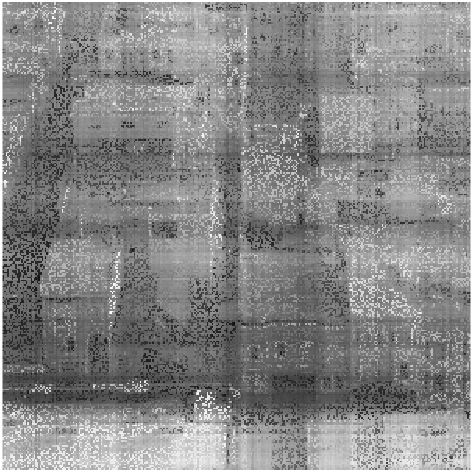
\includegraphics[width=\linewidth]{\mapa/rezLMaFit1.png}
        \caption{Rekonstrukcija s parametrom 1.}
    \end{subfigure}
    \hfill
    \begin{subfigure}{0.325\linewidth}
        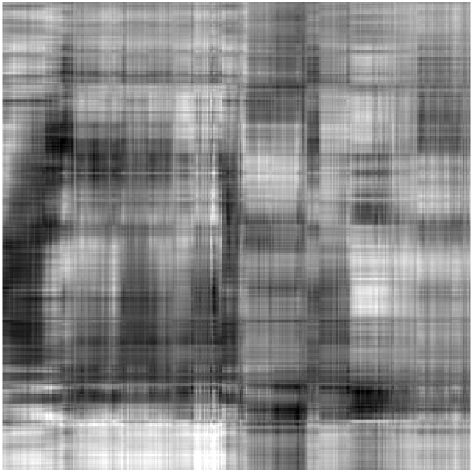
\includegraphics[width=\linewidth]{\mapa/rezLMaFit5.png}
        \caption{Rekonstrukcija s parametrom 5.}
    \end{subfigure}
    \hfill
    \begin{subfigure}{0.325\linewidth}
        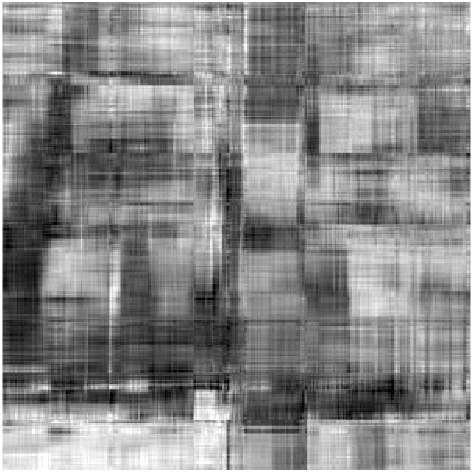
\includegraphics[width=\linewidth]{\mapa/rezLMaFit10.png}
        \caption{Rekonstrukcija s parametrom 10.}
    \end{subfigure}

    \begin{subfigure}{0.325\linewidth}
        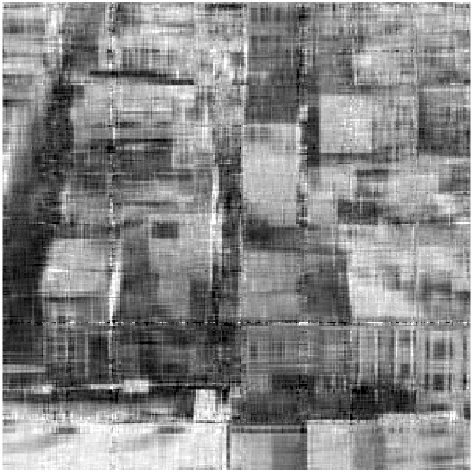
\includegraphics[width=\linewidth]{\mapa/rezLMaFit22.png}
        \caption{Rekonstrukcija s parametrom 22.}
    \end{subfigure}
    \hfill
    \begin{subfigure}{0.325\linewidth}
        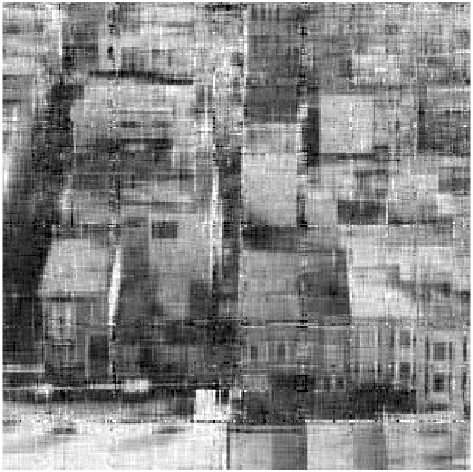
\includegraphics[width=\linewidth]{\mapa/rezLMaFit25.png}
        \caption{Rekonstrukcija s parametrom 25.}
    \end{subfigure}
    \hfill
    \begin{subfigure}{0.325\linewidth}
        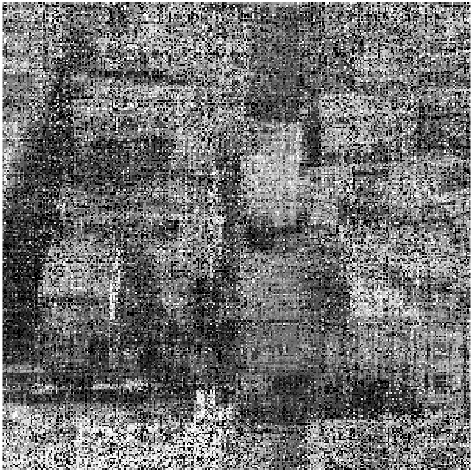
\includegraphics[width=\linewidth]{\mapa/rezLMaFit60.png}
        \caption{Rekonstrukcija s parametrom 60.}
    \end{subfigure}
\end{figure}

\begin{table}[h]
    \centering
    \begin{tabular}{|c|c|c|}
        \hline
        Parameter & Napaka (v $\fnorm{\cdot}$)& Čas izvajanja \\
        \hline
        1         & $1.11 \times 10^4$ & 0.04s        \\
        5         & $8.05 \times 10^3$ & 0.41s         \\
        10        & $6.61 \times 10^3$ & 0.42s        \\
        22        & $6.25 \times 10^3$ & 8.78s       \\
        25        & $6.57 \times 10^3$ & 41.26s        \\
        60        & $2.40 \times 10^4$ & 325.31s        \\
        \hline
    \end{tabular}
    \caption{Rezultati rekonstrukcije algoritma LMaFit za različne parametre.}
\end{table}


Opazimo lahko izboljševanje podrobnosti slike, vse do parametra $22$. Vidimo pa lahko tudi, da pride pri prevelikem parametru do preobrata. Rezultati se ponovno slabšajo, algoritem pa postane počasnejši. Iz tega lahko razberemo, da je pravilna izbira parametra ključna. Vredno je omeniti, da za vrednosti parametra na nekem intervalu algoritem ne konvergira. V primeru zgornje slike in parametra $30$, algoritem LMaFit ni našel rešitve. 

\subsection{TNNM}
Zaradi večje časovne zahtevnosti, algoritem TNNM testiramo zgolj trikrat, na deležih informacij $1, 5$ in $12$. Za večje parametre je algoritem konvergiral zelo počasi, zaradi česar se testiranjem teh izognemo. Tukaj se je pomembno spomniti, da parameter pri algoritmu TNNM ne določa samega ranga rezultata, vendar je zgolj povezan z njim pri reševanju, saj uporablja matriki $A_l$ in $B_l$. Zaradi tega je težje določiti pravilo, kateri parameter je najboljši.
\renewcommand{\mapa}{Poglavja/Slike/informacija ranga}
\begin{figure}[!ht]
    \begin{subfigure}{0.325\linewidth}
        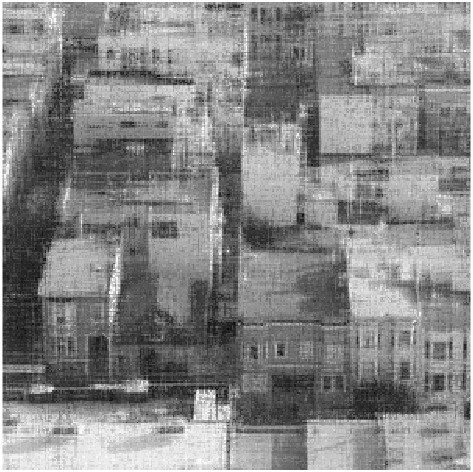
\includegraphics[width=\linewidth]{\mapa/rezTNNM1.png}
        \caption{Rekonstrukcija s parametrom 1.}
    \end{subfigure}
    \hfill
    \begin{subfigure}{0.325\linewidth}
        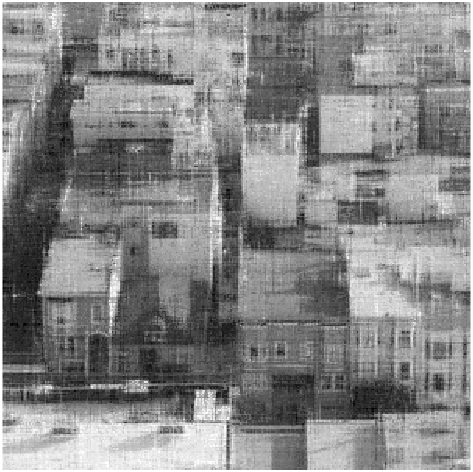
\includegraphics[width=\linewidth]{\mapa/rezTNNM5.png}
        \caption{Rekonstrukcija s parametrom 5.}
    \end{subfigure}
    \hfill
    \begin{subfigure}{0.325\linewidth}
        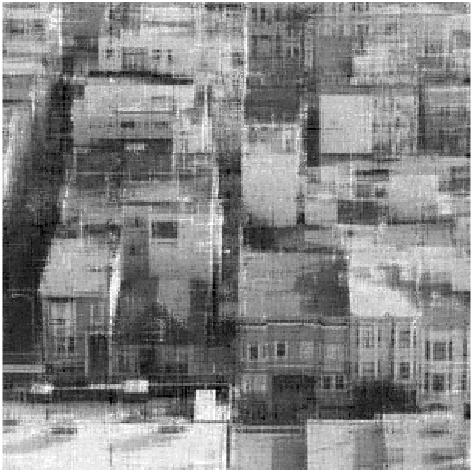
\includegraphics[width=\linewidth]{\mapa/rezTNNM12.png}
        \caption{Rekonstrukcija s parametrom 12.}
    \end{subfigure}
\end{figure}

\begin{figure}[h]
    \centering
    \begin{tabular}{|c|c|c|}
        \hline
        Parameter & Napaka (v $\fnorm{\cdot}$) & Čas izvajanja \\
        \hline
        1 & $5.70 \times 10^{3}$ & 35.9s \\
        5 & $5.46 \times 10^{3}$ & 481s \\
        12 & $5.27 \times 10^{3}$ & 930s \\
        \hline
    \end{tabular}
    \caption{Rezultati rekonstrukcije algoritma TNNM za različne parametre.}
\end{figure}


Sami rezultati med seboj delujejo podobni. Izračun napak nam pokaže, da medtem ko se napaka zmanjšuje s povečevanjem ranga, se hitreje povečuje tudi sam čas reševanja. Torej je treba razmisliti, kako dober rezultat potrebujemo, saj je sama točnost rekonstrukcije časovno draga. Seveda pa velja povedati, da je že pri parametru $1$ TNNM dosegel najboljše rezultate izmed algoritmov v tej diplomski nalogi.

\section{Rekonstrukcija slike z besedilom}
V tem podpoglavju bomo preizkušali učinkovitost algoritmov na slikah, kjer se želimo znebiti besedila na sliki. Gre za drugačno vrsto šuma, kjer namesto da bi bili neznani podatki enakomerno razporejeni, so ti zgoščeni na določenem delu. V našem primeru je bil delež znanih podatkov enak $0.92$, več kot v primerih, ki smo si jih ogledali do sedaj.
\renewcommand{\mapa}{Poglavja/Slike/besedilo}

\begin{figure}[!ht]
    \centering
    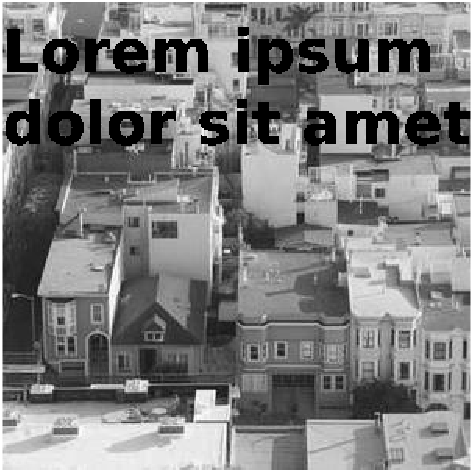
\includegraphics[width=0.32\linewidth]{\mapa/input.png}
    \caption{Slika z besedilom}
\end{figure}

\begin{figure}[!ht]
    \begin{subfigure}{0.325\linewidth}
        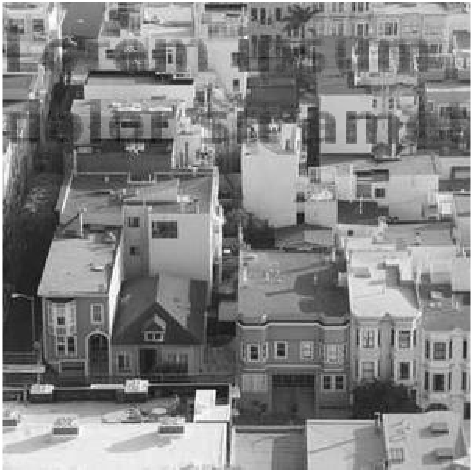
\includegraphics[width=\linewidth]{\mapa/rezSVT.png}
        \caption{Rekonstrukcija z algoritmom SVT}
    \end{subfigure}
    \hfill
    \begin{subfigure}{0.325\linewidth}
        \includegraphics[width=\linewidth]{\mapa/rezTNNM.png}
        \caption{Rekonstrukcija z algoritmom TNNM}
    \end{subfigure}
    \hfill
    \begin{subfigure}{0.325\linewidth}
        \includegraphics[width=\linewidth]{\mapa/rezLMaFit.png}
        \caption{Rekonstrukcija z algoritmom LMaFit}
    \end{subfigure}
\end{figure}

\begin{table}[!ht]
    \centering
    \begin{tabular}{|c|c|c|}
    \hline
    & Napaka & Čas izvajanja (s) \\
    \hline
    SVT & $4.64 \times 10^{3}$ & 674 \\
    TNNM & $2.64 \times 10^{3}$ & 83.6 \\
    LMaFit & $9.10 \times 10^{3}$ & 57.9 \\
    \hline
    \end{tabular}
\end{table}

Ponovno lahko opazimo, da je najboljši rezultat vrnil algoritem TNNM. Pri algoritmu SVT lahko opazimo sledi besedila, zaradi česar je tudi sama napaka pri tem algoritmu večja. Algoritem LMaFit ni skonvergiral za parameter ranga večjega od 16, zaradi česar je sam rezultat produkta matrik $X$ in $Y$ slab. Po vstavitvi  manjkajočih vrednosti seveda večina slike izgleda pravilno, še vedno pa je mogoče razvideti besedilo. 
Rezultati teh testov nam pokažejo pomembnost vrste šuma, saj kljub velikemu deležu znanih podatkov, algoritmi večine podatkov ne morejo kakovostno uporabiti.

\section{Primerjava rezultatov z algoritmom za reševanje Poissonove enačbe}
\todo{Preveri}
Slike se v praksi pogosto rekonstruira z reševanjem Poissonove enačbe
\[
    -\frac{\partial^2v(x, y)}{x^2} - \frac{\partial^2v(x, y)}{y^2} = f(x,y)
\]
kjer odvode zaradi diskretnosti aproksimiramo kot 
\begin{align*}
    -\frac{\partial^2v(x, y)}{x^2} \approx \frac{2v_{i,j} - v_{i-1, j} - v_{i+1, j}}{h^2} \\
    -\frac{\partial^2v(x, y)}{y^2} \approx \frac{2v_{i,j} - v_{i, j-1} - v_{i, j-1}}{h^2}
\end{align*}

Z uporabo Jacobijeve iteracije, lahko problem rešujemo iterativno, tako da neznane vrednosti v vsaki iteraciji posodobimo.
\[
  u_{i, j}^{k+1} = \frac{1}{4}(u_{i - 1, j}^k +  u_{i, j - 1}^k + u_{i + 1, j}^k + u_{i, j + 1}^k)
\]
Spodaj si lahko ogledamo rezultate slik, ponovno preizkušene na sliki mesta.
\renewcommand{\mapa}{Poglavja/Slike/kompleksnost/kompleksna grayscale 300}

\begin{figure}[H]
    \begin{subfigure}{0.32\linewidth}
        \includegraphics[width=\linewidth]{\mapa/rez35Poisson.png}
        \caption{Rekonstrukcija na 0.35 znanih podatkih.}
    \end{subfigure}
    \hfill
    \begin{subfigure}{0.32\linewidth}
        \includegraphics[width=\linewidth]{\mapa/rez45Poisson.png}
        \caption{Rekonstrukcija na 0.45 znanih podatkih.}
    \end{subfigure}
    \hfill
    \begin{subfigure}{0.32\linewidth}
        \includegraphics[width=\linewidth]{\mapa/rez60Poisson.png}
        \caption{Rekonstrukcija na 0.60 znanih podatkih.}
    \end{subfigure}
\end{figure}

\begin{figure}[H]
    \includegraphics[width=\linewidth]{\mapa/napakaPoisson.png}
    \caption{Napaka rekonstrukcij slike mesta glede na delež znanih podatkov.}
\end{figure}

\begin{figure}[H]
    \includegraphics[width=\linewidth]{\mapa/casPoisson.png}
    \caption{Čas izvajanja rekonstrukcije slike mesta glede na delež znanih podatkov.}
\end{figure} 

\FloatBarrier

Vidimo, da je algoritem tako hitrejši, kot bolj točen. Vendar, je pri primerjavi potrebno upoštevati, da se tak algoritem zanaša na podobnost lokalnih podatkov. Pri problemu minimizacije ranga, pa se na take podobnosti ne moremo vedno zanašati. Omenili smo že, da lahko algoritem uporabljamo v priporočilnih sistemih. V takem primeru ne moremo uporabljati sosednosti, saj imata lahko uporabnika v sosednjih vrsticah povsem različne preference. Prav tako si je lahko zamisliti sliko, kjer bi reševanje Poissonove enačbe vrnilo slab rezultat. Tak primer je lahko preprosta dvobarvna slika, sestavljena iz več pasov. Očitno je, da ima originalna slika rang 1. 

\renewcommand{\mapa}{Poglavja/Slike/dvobarvna}

\begin{figure}[!ht]
    \centering
    \includegraphics[width=0.32\linewidth]{\mapa/dvobarvna.png}
    \caption{Dvobarvna slika.}
\end{figure}

\begin{figure}[!ht]
    \begin{subfigure}{0.32\linewidth}
        \includegraphics[width=\linewidth]{\mapa/rez35Poisson.png}
        \caption{Rekonstrukcija na 35\% znanih podatkih.}
    \end{subfigure}
    \hfill
    \begin{subfigure}{0.32\linewidth}
        \includegraphics[width=\linewidth]{\mapa/rez45Poisson.png}
        \caption{Rekonstrukcija na 45\% znanih podatkih.}
    \end{subfigure}
    \hfill
    \begin{subfigure}{0.32\linewidth}
        \includegraphics[width=\linewidth]{\mapa/rez60Poisson.png}
        \caption{Rekonstrukcija na 60\% znanih podatkih.}
    \end{subfigure}
\end{figure}

\begin{figure}[!ht]
    \centering
    \includegraphics[width=\linewidth]{\mapa/cas.png}
    \caption{Čas izvajanja rekonstrukcije dvobarvne slike. Na abscisni osi so deleži znanih podatkov slik.}
\end{figure}
\FloatBarrier
Medtem ko so algoritmi SVT, TNNM in LMaFit sliko rekonstruirali točno, je algoritem za reševanje Poissonove enačbe, kot pričakovano, tu imel več težav. Prav tako je algoritem za reševanje v večini primerov potreboval več časa.